% Collaboration patterns — 2x2 axis showing where the 4 patterns sit.
% X-axis: Pre-action ← → Post-symptom
% Y-axis: You probe Claude (top) ← → Claude probes you (bottom)
%
% Pre-mortem and Interview both have Claude probing the human, but at
% different stages (pre-decision vs mid-proposal). Hypothesis Debugging
% and Feynman both have the human probing Claude, again at different
% stages. The axes capture the *direction of inquiry* and the *workflow
% stage* — the two dimensions that distinguish the 4 patterns most cleanly.
\documentclass[tikz,border=4mm]{standalone}
\usepackage{tikz}
\usetikzlibrary{positioning, shapes.geometric, arrows.meta}

\begin{document}
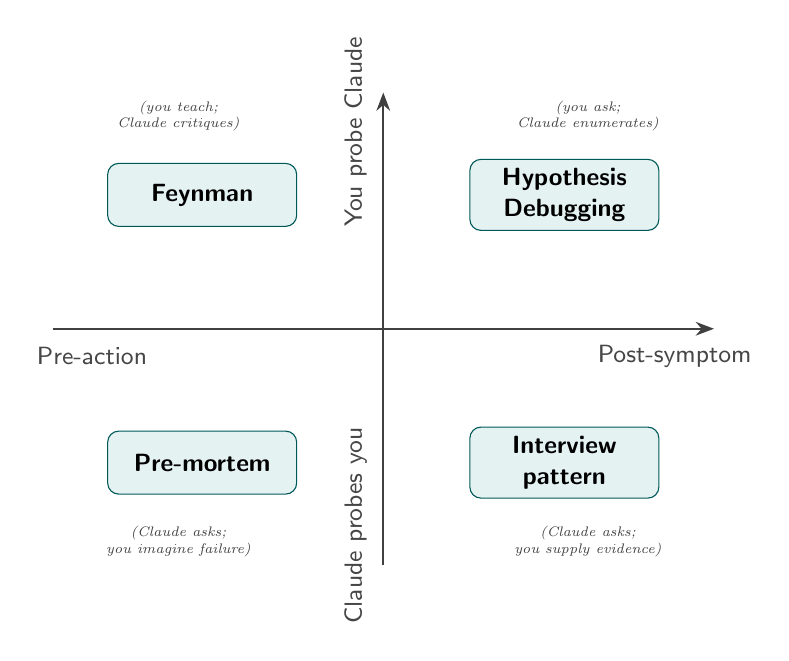
\begin{tikzpicture}[
  font=\sffamily,
  pattern/.style={
    draw=teal!70!black, fill=teal!10, rounded corners=4pt,
    minimum width=2.4cm, minimum height=0.8cm, align=center,
    font=\sffamily\small\bfseries
  },
  axislabel/.style={font=\sffamily\small, text=gray!55!black},
  axisarrow/.style={-Stealth, thick, draw=gray!50!black},
  quadhint/.style={font=\tiny\itshape, text=gray!50!black, align=center},
]

% Axes (X horizontal, Y vertical) centered on origin
\draw[axisarrow] (-4.2, 0) -- (4.2, 0);
\draw[axisarrow] (0, -3.0) -- (0, 3.0);

% Axis end-labels
\node[axislabel] at (-3.7, -0.35) {Pre-action};
\node[axislabel] at (3.7, -0.35) {Post-symptom};
\node[axislabel, rotate=90] at (-0.35, 2.5) {You probe Claude};
\node[axislabel, rotate=90] at (-0.35, -2.5) {Claude probes you};

% Quadrant tag rows (subtle hints)
\node[quadhint] at (-2.6, 2.7) {(you teach;\\Claude critiques)};
\node[quadhint] at (2.6, 2.7) {(you ask;\\Claude enumerates)};
\node[quadhint] at (-2.6, -2.7) {(Claude asks;\\you imagine failure)};
\node[quadhint] at (2.6, -2.7) {(Claude asks;\\you supply evidence)};

% Patterns plotted in the appropriate quadrants
\node[pattern] at (-2.3, 1.7) (feynman) {Feynman};
\node[pattern] at (2.3, 1.7) (hyp) {Hypothesis\\Debugging};
\node[pattern] at (-2.3, -1.7) (pre) {Pre-mortem};
\node[pattern] at (2.3, -1.7) (interview) {Interview\\pattern};

\end{tikzpicture}
\end{document}
